\chapter*{付録}
\label{chap:appendix}
\fancyhf{}
\rhead{\thepage}
\lhead{付録:タグ関係ネットワークにおける抽出タグと既存タグの対応関係}
\cfoot{\thepage}


タグ関係ネットワークにおける抽出タグと既存タグの対応関係

\setcounter{LTchunksize}{10}

\begin{longtable}[c]{|c|c|l|}
\caption{「ASSISTments 2009-2010」}
\label{tab:result1}
\\
%------ 最初のページの表の最上部 ----
\hline
抽出タグ &  TF-IDF値 & 既存タグ\\
\hline
\hline
\endfirsthead
%------ 2ページ以降の表の最上部 ----
\multicolumn{3}{l}{\small\it 前ページからの続き}\\
\hline
抽出タグ &  TF-IDF値 & 既存タグ\\
\hline
\hline
\endhead
%----- ページの表の最下部 --------
\hline
\multicolumn{3}{r}{\small\it 次ページに続く}\\
\endfoot
%----- 最終ページの表の最下部 --------
\hline
\multicolumn{3}{r}{\small\it 以上}\\
\endlastfoot
%----------------------------------------------------------------
\multirow{1}{*}{0} & 1.076 & Addition and Subtraction Integers \\
\hline
\multirow{4}{*}{1} & 0.172 & Probability of a Single Event \\
 & 0.172 & Addition and Subtraction Fractions \\
 & 0.172 & Addition and Subtraction Integers \\
 & 0.080 & Calculations with Similar Figures \\
\hline
\multirow{5}{*}{2} & 0.154 & Addition and Subtraction Fractions \\
 & 0.136 & Probability of a Single Event \\
 & 0.104 & Absolute Value \\
 & 0.050 & Ordering Positive Decimals \\
 & 0.033 & Scientific Notation \\
\hline
\multirow{6}{*}{3} & 0.209 & Probability of a Single Event \\
 & 0.096 & Box and Whisker \\
 & 0.082 & Median \\
 & 0.075 & Pythagorean Theorem \\
 & 0.047 & Write Linear Equation from Ordered Pairs \\
 & 0.038 & Volume Cylinder \\
\hline
\multirow{4}{*}{4} & 0.254 & Addition and Subtraction Fractions \\
 & 0.181 & Probability of a Single Event \\
 & 0.089 & Percent Of \\
 & 0.055 & Order of Operations +,-,/,* () positive reals \\
\hline
\multirow{4}{*}{5} & 0.143 & Probability of a Single Event \\
 & 0.106 & Table \\
 & 0.094 & Mean \\
 & 0.064 & Range \\
\hline
\multirow{3}{*}{6} & 0.198 & Addition and Subtraction Fractions \\
 & 0.184 & Probability of a Single Event \\
 & 0.149 & Percent Of \\
\hline
\multirow{4}{*}{7} & 0.146 & Addition and Subtraction Fractions \\
 & 0.134 & Probability of a Single Event \\
 & 0.115 & Multiplication Fractions \\
 & 0.061 & Scatter Plot \\
\hline
\multirow{3}{*}{8} & 0.252 & Addition and Subtraction Fractions \\
 & 0.185 & Probability of a Single Event \\
 & 0.141 & Percent Of \\
\hline
\multirow{3}{*}{9} & 0.280 & Addition and Subtraction Fractions \\
 & 0.135 & Probability of a Single Event \\
 & 0.085 & Percent Of \\
\hline
\multirow{3}{*}{10} & 0.138 & Absolute Value \\
 & 0.092 & Probability of a Single Event \\
 & 0.091 & Conversion of Fraction Decimals Percents \\
\hline
\multirow{3}{*}{11} & 0.185 & Probability of a Single Event \\
 & 0.167 & Addition and Subtraction Integers \\
 & 0.135 & Equation Solving Two or Fewer Steps \\
\hline
\multirow{4}{*}{12} & 0.188 & Addition and Subtraction Fractions \\
 & 0.162 & Probability of a Single Event \\
 & 0.083 & Box and Whisker \\
 & 0.040 & Interpreting Coordinate Graphs  \\
\hline
\multirow{3}{*}{13} & 0.436 & Probability of a Single Event \\
 & 0.215 & Percent Of \\
 & 0.064 & Median \\
\hline
\multirow{3}{*}{14} & 0.118 & Addition and Subtraction Fractions \\
 & 0.085 & Addition and Subtraction Positive Decimals \\
 & 0.079 & Order of Operations All \\
\hline
\multirow{3}{*}{15} & 0.237 & Probability of a Single Event \\
 & 0.174 & Addition and Subtraction Positive Decimals \\
 & 0.136 & Percent Of \\
\hline
\multirow{4}{*}{16} & 0.184 & Pattern Finding  \\
 & 0.125 & Subtraction Whole Numbers \\
 & 0.110 & Equation Solving Two or Fewer Steps \\
 & 0.076 & Multiplication and Division Integers \\
\hline
\multirow{3}{*}{17} & 0.217 & Addition and Subtraction Positive Decimals \\
 & 0.194 & Probability of a Single Event \\
 & 0.136 & Conversion of Fraction Decimals Percents \\
\hline
\multirow{3}{*}{18} & 0.237 & Probability of a Single Event \\
 & 0.154 & Addition and Subtraction Fractions \\
 & 0.090 & Box and Whisker \\
\hline
\multirow{3}{*}{19} & 0.110 & Probability of a Single Event \\
 & 0.085 & Addition and Subtraction Fractions \\
 & 0.085 & Addition and Subtraction Integers \\
\hline
\multirow{3}{*}{20} & 0.220 & Addition and Subtraction Fractions \\
 & 0.105 & Probability of a Single Event \\
 & 0.100 & Percent Of \\
\hline
\multirow{5}{*}{21} & 0.230 & Probability of a Single Event \\
 & 0.146 & Conversion of Fraction Decimals Percents \\
 & 0.080 & Equation Solving Two or Fewer Steps \\
 & 0.046 & Area Irregular Figure \\
 & 0.045 & Square Root \\
\hline
\multirow{3}{*}{22} & 0.188 & Probability of a Single Event \\
 & 0.108 & Addition and Subtraction Fractions \\
 & 0.088 & Median \\
\hline
\multirow{6}{*}{23} & 0.183 & Finding Percents \\
 & 0.146 & Pattern Finding  \\
 & 0.118 & Addition and Subtraction Positive Decimals \\
 & 0.040 & Effect of Changing Dimensions of a Shape Prportionally \\
 & 0.011 & Perimeter of a Polygon \\
 & 0.011 & Stem and Leaf Plot \\
\hline
\multirow{5}{*}{24} & 0.164 & Equation Solving Two or Fewer Steps \\
 & 0.100 & Addition and Subtraction Integers \\
 & 0.091 & Table \\
 & 0.052 & Fraction Of \\
 & 0.046 & Mode \\
\hline
\multirow{1}{*}{25} & 1.076 & Addition and Subtraction Integers \\
\hline
\multirow{4}{*}{26} & 0.198 & Probability of a Single Event \\
 & 0.132 & Addition and Subtraction Fractions \\
 & 0.094 & Box and Whisker \\
 & 0.051 & Area Trapezoid \\
\hline
\multirow{4}{*}{27} & 0.201 & Probability of a Single Event \\
 & 0.132 & Addition and Subtraction Fractions \\
 & 0.092 & Box and Whisker \\
 & 0.064 & Divisibility Rules \\
\hline
\multirow{3}{*}{28} & 0.205 & Probability of a Single Event \\
 & 0.205 & Addition and Subtraction Fractions \\
 & 0.092 & Box and Whisker \\
\hline
\multirow{3}{*}{29} & 0.191 & Probability of a Single Event \\
 & 0.096 & Percent Of \\
 & 0.091 & Addition and Subtraction Fractions \\
\hline
\multirow{4}{*}{30} & 0.204 & Addition and Subtraction Fractions \\
 & 0.133 & Probability of a Single Event \\
 & 0.110 & Conversion of Fraction Decimals Percents \\
 & 0.091 & Ordering Fractions \\
\hline
\multirow{2}{*}{31} & 0.931 & Write Linear Equation from Graph \\
 & 0.359 & Addition and Subtraction Integers \\
\hline
\multirow{4}{*}{32} & 0.236 & Probability of a Single Event \\
 & 0.202 & Percent Of \\
 & 0.147 & Addition and Subtraction Fractions \\
 & 0.062 & Addition Whole Numbers \\
\hline
\multirow{3}{*}{33} & 0.230 & Addition and Subtraction Positive Decimals \\
 & 0.097 & Order of Operations All \\
 & 0.076 & Conversion of Fraction Decimals Percents \\
\hline
\multirow{3}{*}{34} & 0.227 & Probability of a Single Event \\
 & 0.191 & Addition and Subtraction Fractions \\
 & 0.139 & Percent Of \\
\hline
\multirow{3}{*}{35} & 0.173 & Probability of a Single Event \\
 & 0.135 & Addition and Subtraction Fractions \\
 & 0.113 & Addition and Subtraction Integers \\
\hline
\multirow{4}{*}{36} & 0.189 & Probability of a Single Event \\
 & 0.189 & Addition and Subtraction Fractions \\
 & 0.096 & Percent Of \\
 & 0.036 & Estimation \\
\hline
\multirow{3}{*}{37} & 0.264 & Probability of a Single Event \\
 & 0.244 & Addition and Subtraction Fractions \\
 & 0.193 & Percent Of \\
\hline
\multirow{4}{*}{38} & 0.223 & Pattern Finding  \\
 & 0.152 & Subtraction Whole Numbers \\
 & 0.109 & Finding Percents \\
 & 0.050 & Histogram as Table or Graph \\
\hline
\multirow{3}{*}{39} & 0.158 & Probability of a Single Event \\
 & 0.130 & Addition and Subtraction Fractions \\
 & 0.108 & Percent Of \\
\hline
\multirow{3}{*}{40} & 0.258 & Addition and Subtraction Fractions \\
 & 0.167 & Probability of a Single Event \\
 & 0.130 & Box and Whisker \\
\hline
\multirow{3}{*}{41} & 0.302 & Finding Percents \\
 & 0.189 & Addition and Subtraction Positive Decimals \\
 & 0.099 & Conversion of Fraction Decimals Percents \\
\hline
\multirow{3}{*}{42} & 0.121 & Addition and Subtraction Positive Decimals \\
 & 0.111 & Probability of a Single Event \\
 & 0.090 & Addition and Subtraction Fractions \\
\hline
\multirow{3}{*}{43} & 0.249 & Probability of a Single Event \\
 & 0.184 & Addition and Subtraction Fractions \\
 & 0.125 & Percent Of \\
\hline
\multirow{3}{*}{44} & 0.247 & Addition and Subtraction Fractions \\
 & 0.129 & Probability of a Single Event \\
 & 0.108 & Percent Of \\
\hline
\multirow{3}{*}{45} & 0.212 & Probability of a Single Event \\
 & 0.173 & Addition and Subtraction Fractions \\
 & 0.100 & Box and Whisker \\
\hline
\multirow{3}{*}{46} & 0.204 & Probability of a Single Event \\
 & 0.185 & Addition and Subtraction Fractions \\
 & 0.118 & Percent Of \\
\hline
\multirow{4}{*}{47} & 0.326 & Surface Area Rectangular Prism \\
 & 0.272 & Pattern Finding  \\
 & 0.205 & Equation Solving More Than Two Steps \\
 & 0.175 & Venn Diagram \\
\hline
\multirow{3}{*}{48} & 0.145 & Probability of a Single Event \\
 & 0.129 & Equation Solving Two or Fewer Steps \\
 & 0.099 & Addition and Subtraction Fractions \\
\hline
\multirow{5}{*}{49} & 0.145 & Addition and Subtraction Positive Decimals \\
 & 0.081 & Equation Solving Two or Fewer Steps \\
 & 0.064 & Equivalent Fractions \\
 & 0.061 & Division Fractions \\
 & 0.034 & Volume Sphere \\
\hline
\multirow{5}{*}{50} & 0.111 & Probability of a Single Event \\
 & 0.111 & Addition and Subtraction Integers \\
 & 0.090 & Probability of Two Distinct Events \\
 & 0.074 & Counting Methods \\
 & 0.071 & Proportion \\
\hline
\multirow{3}{*}{51} & 0.134 & Equation Solving Two or Fewer Steps \\
 & 0.121 & Addition and Subtraction Positive Decimals \\
 & 0.115 & Probability of a Single Event \\
\hline
\multirow{5}{*}{52} & 0.175 & Probability of a Single Event \\
 & 0.128 & Percent Of \\
 & 0.081 & Addition and Subtraction Fractions \\
 & 0.079 & Circle Graph \\
 & 0.054 & Unit Rate \\
\hline
\multirow{5}{*}{53} & 0.372 & Equation Solving Two or Fewer Steps \\
 & 0.203 & Order of Operations All \\
 & 0.130 & Probability of a Single Event \\
 & 0.073 & Least Common Multiple \\
 & 0.072 & Circumference  \\
\hline
\multirow{2}{*}{54} & 0.538 & Probability of a Single Event \\
 & 0.538 & Addition and Subtraction Fractions \\
\hline
\end{longtable}


\begin{longtable}[c]{|c|c|l|}
\caption{「Bridge to Algebra 2006-2007」}
\label{tab:result1}
\\
%------ 最初のページの表の最上部 ----
\hline
抽出タグ &  TF-IDF値 & 既存タグ\\
\hline
\hline
\endfirsthead
%------ 2ページ以降の表の最上部 ----
\multicolumn{3}{l}{\small\it 前ページからの続き}\\
\hline
抽出タグ &  TF-IDF値 & 既存タグ\\
\hline
\hline
\endhead
%----- ページの表の最下部 --------
\hline
\multicolumn{3}{r}{\small\it 次ページに続く}\\
\endfoot
%----- 最終ページの表の最下部 --------
\hline
\multicolumn{3}{r}{\small\it 以上}\\
\endlastfoot
%----------------------------------------------------------------
\multirow{3}{*}{\small 0} & \small 0.388 & \small Identify common denominator \\
 & \small 0.344 & \small Rewrite fraction with common denominator \\
 & \small 0.290 & \small Identify number of equal divisions on number line from desired denominator \\
\hline
\multirow{3}{*}{\small 1} & \small 0.707 & \small Identify Fraction using fraction shape \\
 & \small 0.561 & \small Calculate product of two numbers \\
 & \small 0.561 & \small Identify GCF in written question \\
\hline
\multirow{3}{*}{\small 2} & \small 0.842 & \small Enter smaller inital in diagram -- calculated \\
 & \small 0.774 & \small Draw larger bar -- addition/subtraction \\
 & \small 0.726 & \small Identify number of desired groups \\
\hline
\multirow{3}{*}{\small 3} & \small 0.442 & \small Calculate difference with positive integer \\
 & \small 0.357 & \small Identify multiplier in written question -- number line \\
 & \small 0.304 & \small Identify fraction associated with each piece of a square \\
\hline
\multirow{3}{*}{\small 4} & \small 0.774 & \small Draw larger bar -- addition/subtraction \\
 & \small 0.689 & \small Draw smaller bar -- addition/subtraction \\
 & \small 0.518 & \small Identify multiplier in equivalence statement \\
\hline
\multirow{3}{*}{\small 5} & \small 0.383 & \small Identify number as common factor \\
 & \small 0.293 & \small Identify number of items \\
 & \small 0.220 & \small Calculate Part \\
\hline
\multirow{3}{*}{\small 6} & \small 0.574 & \small Represent multiplier visually \\
 & \small 0.574 & \small Calculate product -- multiply statement \\
 & \small 0.355 & \small Label equivalent fraction on number line \\
\hline
\multirow{3}{*}{\small 7} & \small 0.574 & \small Identify equal parts for multiplier \\
 & \small 0.440 & \small Identify number as common factor \\
 & \small 0.436 & \small Enter subtracted quantity in diagram \\
\hline
\multirow{2}{*}{\small 8} & \small 1.590 & \small List consecutive multiples of a number \\
 & \small 0.734 & \small Identify number as common factor \\
\hline
\multirow{3}{*}{\small 9} & \small 1.436 & \small Identify that a fraction can/cannot be simplified \\
 & \small 1.090 & \small Enter items denominator \\
 & \small 0.837 & \small Identify larger quantity -- multiplication \\
\hline
\multirow{3}{*}{\small 10} & \small 0.957 & \small Identify whole number of improper fraction symbolically \\
 & \small 0.734 & \small Identify number as common factor \\
 & \small 0.726 & \small Identify fractional part of improper fraction symbolically \\
\hline
\multirow{3}{*}{\small 11} & \small 0.611 & \small Rewrite fraction with common denominator \\
 & \small 0.536 & \small Identify LCM - is product \\
 & \small 0.407 & \small Compare fractions with like denominators \\
\hline
\multirow{3}{*}{\small 12} & \small 0.410 & \small Identify width of overlap \\
 & \small 0.332 & \small Identify number of equal divisions on number line from desired denominator \\
 & \small 0.311 & \small Represent second fraction on number line as difference \\
\hline
\multirow{3}{*}{\small 13} & \small 1.149 & \small Represent negative integer using number line \\
 & \small 0.733 & \small Enter added quantity in diagram \\
 & \small 0.550 & \small Identify improper fraction from option 2 \\
\hline
\multirow{3}{*}{\small 14} & \small 1.090 & \small Calculate sum -- contextual \\
 & \small 0.861 & \small Count number of shaded parts in square (discontiguous) \\
 & \small 0.728 & \small Draw larger bar -- multiplication \\
\hline
\multirow{3}{*}{\small 15} & \small 1.684 & \small Identify number of equal divisions in visual from fraction \\
 & \small 0.720 & \small Identify number of recipients \\
 & \small 0.489 & \small Identify number as common factor \\
\hline
\multirow{3}{*}{\small 16} & \small 0.957 & \small Rewrite adding positive integer \\
 & \small 0.842 & \small Represent first integer on number line \\
 & \small 0.720 & \small Identify number of recipients \\
\hline
\multirow{2}{*}{\small 17} & \small 2.526 & \small Identify number of equal divisions (vertical bar) \\
 & \small 0.734 & \small Identify number as common factor \\
\hline
\multirow{3}{*}{\small 18} & \small 0.957 & \small Identify number of desired groups--construct \\
 & \small 0.720 & \small Identify number of recipients \\
 & \small 0.485 & \small Draw larger bar -- multiplication \\
\hline
\multirow{3}{*}{\small 19} & \small 1.090 & \small Identify number of desired groups \\
 & \small 1.034 & \small Identify negative integer from number line \\
 & \small 0.795 & \small Identify Fraction using fraction shape \\
\hline
\multirow{3}{*}{\small 20} & \small 0.718 & \small Represent multiplicand visually \\
 & \small 0.718 & \small Identify fraction associated with each piece of a horizontal bar \\
 & \small 0.652 & \small Identify improper fraction from option 1 \\
\hline
\multirow{3}{*}{\small 21} & \small 1.436 & \small Draw smaller bar -- multiplication \\
 & \small 1.263 & \small Identify fraction of desired items \\
 & \small 1.263 & \small Identify fraction associated with each piece of a circle \\
\hline
\multirow{1}{*}{\small 22} & \small 3.953 & \small Calculate sum -- non contextual \\
\hline
\multirow{3}{*}{\small 23} & \small 0.734 & \small Identify number as common factor \\
 & \small 0.689 & \small Identify number of equal groups from fraction \\
 & \small 0.485 & \small List factor of large number \\
\hline
\multirow{3}{*}{\small 24} & \small 0.971 & \small Draw larger bar -- multiplication \\
 & \small 0.749 & \small Identify number of items \\
 & \small 0.489 & \small Identify number as common factor \\
\hline
\multirow{2}{*}{\small 25} & \small 2.179 & \small Identify number of items in each group \\
 & \small 1.456 & \small List factor of large number \\
\hline
\multirow{3}{*}{\small 26} & \small 0.821 & \small Identify larger quantity -- subtraction \\
 & \small 0.722 & \small Identify GCF in written question \\
 & \small 0.629 & \small Identify number as common factor \\
\hline
\multirow{3}{*}{\small 27} & \small 1.436 & \small Identify whole number upper bound \\
 & \small 1.263 & \small Identify number of equal divisions (circle) \\
 & \small 1.090 & \small Identify fractional part of improper fraction symbolically \\
\hline
\multirow{3}{*}{\small 28} & \small 0.774 & \small Identify multiplier in written question -- rectangle \\
 & \small 0.726 & \small Enter subtracted quantity in diagram \\
 & \small 0.633 & \small Label equivalent fraction in equivalence statement \\
\hline
\multirow{2}{*}{\small 29} & \small 2.872 & \small Write improper fraction as mixed number \\
 & \small 1.833 & \small Compare fractions with like denominators \\
\hline
\multirow{3}{*}{\small 30} & \small 1.222 & \small Calculate difference -- contextual \\
 & \small 0.957 & \small Identify GCF \\
 & \small 0.842 & \small Calculate difference -- non contextual \\
\hline
\multirow{3}{*}{\small 31} & \small 1.010 & \small Enter smaller inital in diagram -- calculated \\
 & \small 0.760 & \small Represent first fraction on number line \\
 & \small 0.550 & \small Rewrite fraction with common denominator \\
\hline
\multirow{2}{*}{\small 32} & \small 2.526 & \small Calculate Total \\
 & \small 1.206 & \small Identify LCM - is product \\
\hline
\multirow{3}{*}{\small 33} & \small 0.383 & \small Identify whole number lower bound \\
 & \small 0.337 & \small Identify fraction associated with each piece of a vertical bar \\
 & \small 0.294 & \small Identify number as common factor \\
\hline
\multirow{2}{*}{\small 34} & \small 1.305 & \small Identify improper fraction from option 1 \\
 & \small 1.124 & \small Identify number of items \\
\hline
\multirow{3}{*}{\small 35} & \small 0.916 & \small Identify GCF - one number multiple of other \\
 & \small 0.687 & \small Identify improper fraction from option 2 \\
 & \small 0.603 & \small Identify LCM - is product \\
\hline
\multirow{3}{*}{\small 36} & \small 0.397 & \small Identify number of items \\
 & \small 0.338 & \small Enter smaller initial in diagram -- given \\
 & \small 0.323 & \small Compare Options - operation \\
\hline
\multirow{1}{*}{\small 37} & \small 2.161 & \small Identify number of recipients \\
\hline
\multirow{3}{*}{\small 38} & \small 1.149 & \small Write mixed number as improper fraction \\
 & \small 0.760 & \small Represent first fraction on number line \\
 & \small 0.710 & \small Label equivalent fraction on number line \\
\hline
\multirow{3}{*}{\small 39} & \small 0.409 & \small Identify number of items \\
 & \small 0.396 & \small Represent second fraction on number line as difference \\
 & \small 0.393 & \small Identify number of recipients \\
\hline
\multirow{3}{*}{\small 40} & \small 0.454 & \small Identify Fraction using fraction shape \\
 & \small 0.321 & \small Identify number of items \\
 & \small 0.315 & \small Identify number as common factor \\
\hline
\multirow{3}{*}{\small 41} & \small 1.553 & \small Identify multiplier in equivalence statement \\
 & \small 0.652 & \small Identify improper fraction from option 1 \\
 & \small 0.367 & \small Identify number as common factor \\
\hline
\multirow{3}{*}{\small 42} & \small 0.718 & \small Identify equal parts for multiplicand \\
 & \small 0.545 & \small Calculate sum -- contextual \\
 & \small 0.540 & \small Identify number of recipients \\
\hline
\multirow{1}{*}{\small 43} & \small 2.609 & \small Identify improper fraction from option 1 \\
\hline
\multirow{3}{*}{\small 44} & \small 1.263 & \small Calculate Part \\
 & \small 0.728 & \small Draw larger bar -- multiplication \\
 & \small 0.687 & \small Compare Options - operation \\
\hline
\multirow{3}{*}{\small 45} & \small 0.516 & \small Identify multiplier in written question -- number line \\
 & \small 0.489 & \small Identify number as common factor \\
 & \small 0.459 & \small Identify number of equal groups from fraction \\
\hline
\multirow{1}{*}{\small 46} & \small 1.468 & \small Identify number as common factor \\
\hline
\multirow{3}{*}{\small 47} & \small 0.381 & \small Identify number as common factor \\
 & \small 0.236 & \small List consecutive multiples of a number \\
 & \small 0.213 & \small Identify whole number of mixed number symbolically \\
\hline
\multirow{3}{*}{\small 48} & \small 0.442 & \small Calculate area of overlap \\
 & \small 0.339 & \small Identify number as common factor \\
 & \small 0.335 & \small Compare fractions from contextual problem \\
\hline
\multirow{3}{*}{\small 49} & \small 0.536 & \small Identify LCM - is product \\
 & \small 0.484 & \small Enter items numerator \\
 & \small 0.362 & \small Identify larger quantity -- addition \\
\hline
\multirow{3}{*}{\small 50} & \small 1.010 & \small Identify GCF in equivalence statement \\
 & \small 0.550 & \small Compare Options - operation \\
 & \small 0.550 & \small Identify improper fraction from option 2 \\
\hline
\multirow{3}{*}{\small 51} & \small 0.281 & \small Represent first fraction on number line \\
 & \small 0.250 & \small Identify number of items \\
 & \small 0.240 & \small Identify number of recipients \\
\hline
\multirow{3}{*}{\small 52} & \small 0.451 & \small Calculate sum -- contextual \\
 & \small 0.409 & \small Identify fraction associated with each piece of a square \\
 & \small 0.373 & \small Identify number of recipients \\
\hline
\multirow{3}{*}{\small 53} & \small 0.447 & \small Label equivalent fraction in equivalence statement \\
 & \small 0.397 & \small Identify number of items \\
 & \small 0.345 & \small Identify number as common factor \\
\hline
\multirow{3}{*}{\small 54} & \small 1.149 & \small Represent second positive integer on number line as difference \\
 & \small 0.827 & \small Draw smaller bar -- addition/subtraction \\
 & \small 0.587 & \small Identify number as common factor \\
\hline
\multirow{3}{*}{\small 55} & \small 1.436 & \small Convert improper fraction to whole number \\
 & \small 0.728 & \small List factor of large number \\
 & \small 0.540 & \small Identify number of recipients \\
\hline
\multirow{3}{*}{\small 56} & \small 0.629 & \small Identify number as common factor \\
 & \small 0.543 & \small Enter larger inital in diagram -- calculated \\
 & \small 0.393 & \small Rewrite fraction with common denominator \\
\hline
\multirow{3}{*}{\small 57} & \small 0.722 & \small Identify number of equal divisions in visual from fraction \\
 & \small 0.722 & \small Identify GCF in equivalence statement \\
 & \small 0.524 & \small Compare fractions with unlike denominators \\
\hline
\multirow{3}{*}{\small 58} & \small 0.957 & \small Calculate sum with positive integer \\
 & \small 0.611 & \small Enter added quantity in diagram \\
 & \small 0.458 & \small Identify improper fraction from option 2 \\
\hline
\multirow{3}{*}{\small 59} & \small 0.774 & \small Identify multiplier in written question -- rectangle \\
 & \small 0.726 & \small Enter items numerator \\
 & \small 0.591 & \small Label equivalent fraction on number line \\
\hline
\multirow{3}{*}{\small 60} & \small 0.957 & \small Isolate numerator of fractional part of mixed number symbolically \\
 & \small 0.957 & \small Enter larger initial in diagram -- given \\
 & \small 0.842 & \small Identify fraction of desired items \\
\hline
\multirow{2}{*}{\small 61} & \small 1.206 & \small Identify LCM - is product \\
 & \small 0.734 & \small Identify number as common factor \\
\hline
\multirow{3}{*}{\small 62} & \small 0.581 & \small Identify number of desired items \\
 & \small 0.545 & \small Compare fractions from contextual problem \\
 & \small 0.540 & \small Identify number of recipients \\
\hline
\multirow{3}{*}{\small 63} & \small 1.090 & \small Represent second fraction on number line as sum \\
 & \small 0.652 & \small Identify improper fraction from option 1 \\
 & \small 0.562 & \small Identify number of items \\
\hline
\multirow{2}{*}{\small 64} & \small 1.206 & \small Identify LCM - is product \\
 & \small 0.734 & \small Identify number as common factor \\
\hline
\multirow{3}{*}{\small 65} & \small 0.550 & \small Rewrite fraction with common denominator \\
 & \small 0.392 & \small Identify number as common factor \\
 & \small 0.367 & \small Compare Options - operation \\
\hline
\multirow{3}{*}{\small 66} & \small 0.530 & \small List consecutive multiples of a number \\
 & \small 0.375 & \small Identify number of items \\
 & \small 0.363 & \small Calculate sum -- contextual \\
\hline
\multirow{3}{*}{\small 67} & \small 0.647 & \small List factor of large number \\
 & \small 0.561 & \small Calculate Total \\
 & \small 0.484 & \small Label equivalent fraction in visual \\
\hline
\multirow{3}{*}{\small 68} & \small 0.518 & \small Identify multiplier in equivalence statement \\
 & \small 0.479 & \small Enter quantity from diagram by calculating \\
 & \small 0.345 & \small Identify number of equal groups from fraction \\
\hline
\multirow{3}{*}{\small 69} & \small 1.222 & \small Enter added quantity in diagram \\
 & \small 0.749 & \small Identify number of items \\
 & \small 0.489 & \small Identify number as common factor \\
\hline
\multirow{3}{*}{\small 70} & \small 0.397 & \small Identify number of items \\
 & \small 0.297 & \small Identify number of items in each group from GCF \\
 & \small 0.284 & \small Identify LCM - is product \\
\hline
\multirow{2}{*}{\small 71} & \small 1.553 & \small Identify multiplier in equivalence statement \\
 & \small 1.456 & \small Draw larger bar -- multiplication \\
\hline
\multirow{3}{*}{\small 72} & \small 0.957 & \small Identify number of equal divisions (horizontal bar) \\
 & \small 0.774 & \small Count number of shaded parts in vertical bar (discontiguous) \\
 & \small 0.659 & \small Calculate sum -- non contextual \\
\hline
\multirow{3}{*}{\small 73} & \small 1.034 & \small Identify negative integer from number line \\
 & \small 0.687 & \small Compare Options - operation \\
 & \small 0.652 & \small Identify improper fraction from option 1 \\
\hline
\multirow{1}{*}{\small 74} & \small 2.749 & \small Identify improper fraction from option 2 \\
\hline
\multirow{3}{*}{\small 75} & \small 0.734 & \small Identify number as common factor \\
 & \small 0.611 & \small Identify that a fraction cannot be simplified \\
 & \small 0.485 & \small Draw larger bar -- multiplication \\
\hline
\multirow{3}{*}{\small 76} & \small 0.687 & \small Rewrite fraction with common denominator \\
 & \small 0.631 & \small Identify number of items in each group from GCF \\
 & \small 0.408 & \small Identify larger quantity -- addition \\
\hline
\multirow{3}{*}{\small 77} & \small 0.367 & \small Identify improper fraction from option 2 \\
 & \small 0.367 & \small Rewrite fraction with common denominator \\
 & \small 0.337 & \small Identify fraction associated with each piece of a circle \\
\hline
\multirow{1}{*}{\small 78} & \small 3.665 & \small Compare fractions with unlike denominators \\
\hline
\multirow{3}{*}{\small 79} & \small 0.760 & \small Represent first fraction on number line \\
 & \small 0.733 & \small Identify that a fraction cannot be simplified \\
 & \small 0.621 & \small Identify common denominator \\
\hline
\multirow{3}{*}{\small 80} & \small 1.060 & \small Identify Fraction using fraction shape \\
 & \small 0.971 & \small Draw larger bar -- multiplication \\
 & \small 0.489 & \small Identify number as common factor \\
\hline
\multirow{3}{*}{\small 81} & \small 0.821 & \small Enter total in diagram - calculated - addition \\
 & \small 0.664 & \small Count number of shaded parts in vertical bar (discontiguous) \\
 & \small 0.623 & \small Label equivalent fraction in visual \\
\hline
\multirow{3}{*}{\small 82} & \small 0.707 & \small List consecutive multiples of a number \\
 & \small 0.638 & \small Identify number of total items \\
 & \small 0.561 & \small Identify fraction associated with each piece of a vertical bar \\
\hline
\multirow{3}{*}{\small 83} & \small 1.350 & \small Identify number as common multiple \\
 & \small 1.090 & \small Identify fractional part of improper fraction symbolically \\
 & \small 0.367 & \small Identify number as common factor \\
\hline
\multirow{1}{*}{\small 84} & \small 3.347 & \small Identify larger quantity -- multiplication \\
\hline
\multirow{3}{*}{\small 85} & \small 0.631 & \small Identify proper fraction from option 1 \\
 & \small 0.562 & \small Identify number of items \\
 & \small 0.430 & \small Count number of shaded parts in square (discontiguous) \\
\hline
\multirow{3}{*}{\small 86} & \small 0.827 & \small Draw smaller bar -- addition/subtraction \\
 & \small 0.636 & \small Identify Fraction using fraction shape \\
 & \small 0.636 & \small List consecutive multiples of a number \\
\hline
\multirow{3}{*}{\small 87} & \small 0.842 & \small Identify number of equal divisions (circle) \\
 & \small 0.689 & \small Enter quantity from diagram by reading \\
 & \small 0.633 & \small Enter larger inital in diagram -- calculated \\
\hline
\multirow{3}{*}{\small 88} & \small 1.222 & \small Identify GCF - one number multiple of other \\
 & \small 0.916 & \small Compare Options - operation \\
 & \small 0.804 & \small Identify LCM - is product \\
\hline
\multirow{6}{*}{\small 89} & \small nan & \small Count number of shaded parts in circle (contiguous) \\
 & \small nan & \small Convert whole number to improper fraction \\
 & \small nan & \small Represent second positive integer on number line as sum \\
 & \small nan & \small Enter initial in diagram -- given \\
 & \small nan & \small Write mixed number as improper fraction \\
 & \small nan & \small Enter group denominator \\
\hline
\multirow{2}{*}{\small 90} & \small 2.068 & \small Identify negative integer from number line \\
 & \small 1.674 & \small Identify larger quantity -- multiplication \\
\hline
\multirow{2}{*}{\small 91} & \small 1.590 & \small Identify Fraction using fraction shape \\
 & \small 1.456 & \small List factor of large number \\
\hline
\multirow{3}{*}{\small 92} & \small 0.776 & \small Identify common denominator \\
 & \small 0.540 & \small Identify number of recipients \\
 & \small 0.458 & \small Compare fractions with like denominators \\
\hline
\multirow{3}{*}{\small 93} & \small 0.638 & \small Enter total in diagram - calculated - multiplication \\
 & \small 0.484 & \small Enter group numerator \\
 & \small 0.345 & \small Identify common denominator \\
\hline
\multirow{2}{*}{\small 94} & \small 2.179 & \small Enter items denominator \\
 & \small 0.734 & \small Identify number as common factor \\
\hline
\multirow{1}{*}{\small 95} & \small 3.799 & \small Represent first fraction on number line \\
\hline
\multirow{3}{*}{\small 96} & \small 0.450 & \small Identify number of items \\
 & \small 0.392 & \small Identify number as common factor \\
 & \small 0.310 & \small Count number of shaded parts in vertical bar (discontiguous) \\
\hline
\multirow{1}{*}{\small 97} & \small 3.665 & \small Identify that a fraction cannot be simplified \\
\hline
\multirow{3}{*}{\small 98} & \small 1.178 & \small Compare Options - operation \\
 & \small 0.664 & \small Draw larger bar -- addition/subtraction \\
 & \small 0.524 & \small Identify GCF - one number multiple of other \\
\hline
\multirow{3}{*}{\small 99} & \small 0.522 & \small Identify length of overlap \\
 & \small 0.522 & \small Identify proper fraction from option 2 \\
 & \small 0.359 & \small Identify fraction associated with each piece of a square \\
\hline
\multirow{3}{*}{\small 100} & \small 1.915 & \small Identify fractional part of mixed number symbolically \\
 & \small 0.916 & \small Compare Options - operation \\
 & \small 0.870 & \small Identify improper fraction from option 1 \\
\hline
\multirow{3}{*}{\small 101} & \small 0.611 & \small Enter added quantity in diagram \\
 & \small 0.611 & \small Compare fractions with unlike denominators \\
 & \small 0.530 & \small Identify Fraction using fraction shape \\
\hline
\multirow{1}{*}{\small 102} & \small 1.468 & \small Identify number as common factor \\
\hline
\multirow{3}{*}{\small 103} & \small 1.123 & \small Calculate difference -- non contextual \\
 & \small 0.500 & \small Identify number of items \\
 & \small 0.439 & \small Identify fraction associated with each piece of a square \\
\hline
\multirow{3}{*}{\small 104} & \small 0.957 & \small Copy initial in diagram \\
 & \small 0.957 & \small Compare Options - simplified \\
 & \small 0.543 & \small Identify number of equal divisions (square) \\
\hline
\multirow{1}{*}{\small 105} & \small 3.665 & \small Compare fractions with like denominators \\
\hline
\multirow{3}{*}{\small 106} & \small 0.733 & \small Enter added quantity in diagram \\
 & \small 0.669 & \small Identify larger quantity -- multiplication \\
 & \small 0.550 & \small Rewrite fraction with common denominator \\
\hline
\multirow{3}{*}{\small 107} & \small 0.551 & \small Identify number as common factor \\
 & \small 0.545 & \small Enter subtracted quantity in diagram \\
 & \small 0.458 & \small Compare fractions with unlike denominators \\
\hline
\multirow{3}{*}{\small 108} & \small 0.500 & \small Identify number of items \\
 & \small 0.484 & \small Enter items numerator \\
 & \small 0.484 & \small Enter group denominator \\
\hline
\multirow{3}{*}{\small 109} & \small 0.929 & \small Identify number of equal divisions on number line from desired denominator \\
 & \small 0.636 & \small Identify Fraction using fraction shape \\
 & \small 0.550 & \small Identify improper fraction from option 2 \\
\hline
\multirow{3}{*}{\small 110} & \small 0.611 & \small Compare Options - operation \\
 & \small 0.516 & \small Identify number of desired items \\
 & \small 0.484 & \small Identify number of items in each group \\
\hline
\multirow{3}{*}{\small 111} & \small 1.100 & \small Identify improper fraction from option 2 \\
 & \small 1.010 & \small Count number of shaded parts in square (contiguous) \\
 & \small 0.827 & \small Draw smaller bar -- addition/subtraction \\
\hline
\multirow{3}{*}{\small 112} & \small 0.475 & \small Identify that a fraction can be simplified \\
 & \small 0.359 & \small Enter total in diagram - calculated - subtraction \\
 & \small 0.344 & \small Compare Options - operation \\
\hline
\multirow{3}{*}{\small 113} & \small 0.442 & \small Enter initial in diagram -- given \\
 & \small 0.335 & \small Enter items numerator \\
 & \small 0.335 & \small Enter group numerator \\
\hline
\multirow{3}{*}{\small 114} & \small 0.965 & \small Identify LCM - is product \\
 & \small 0.760 & \small Enter larger inital in diagram -- calculated \\
 & \small 0.733 & \small Compare fractions with like denominators \\
\hline
\end{longtable}


%\begin{figure}[htb]
%\begin{center}
%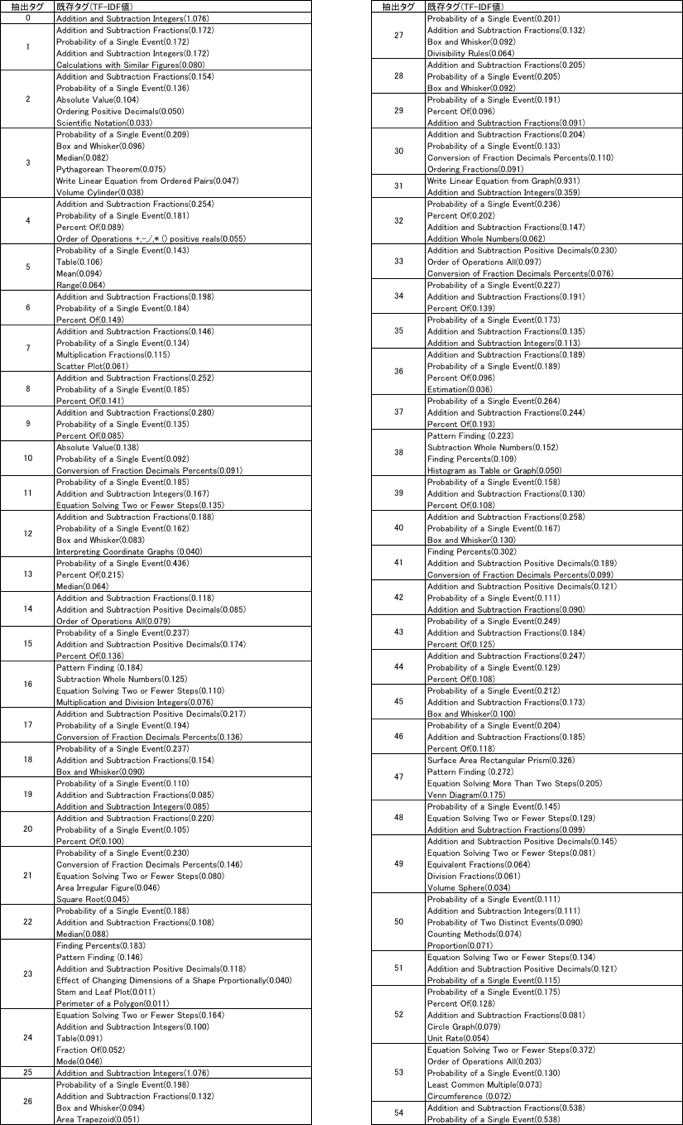
\includegraphics[height=400pt]{./img/aTable.png}
%\end{center}
%\caption{「ASSISTments 2009-2010」の抽出タグと既存タグの対応関係}
%\label{fig:aTable}
%\end{figure}
%
%\begin{figure}[htb]
%\begin{center}
%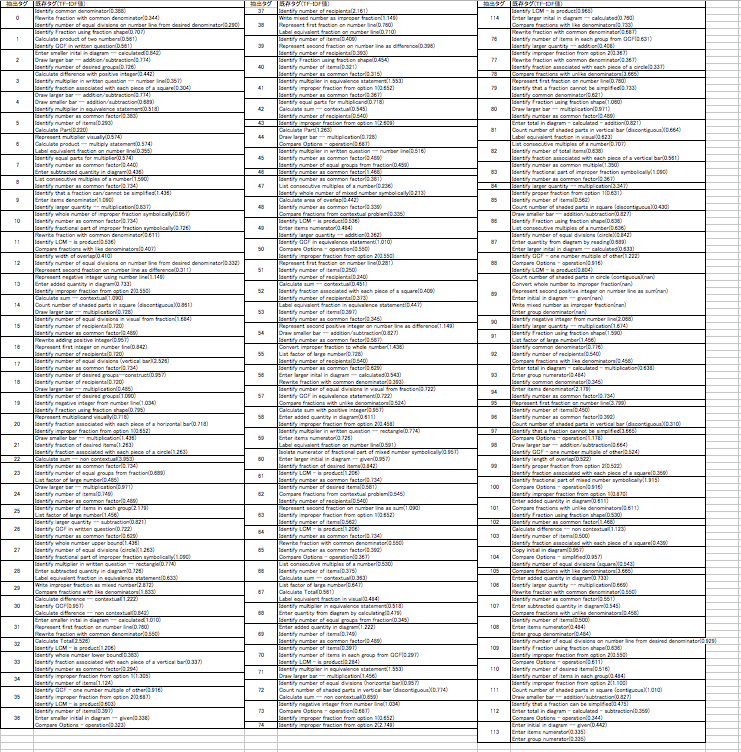
\includegraphics[height=400pt]{./img/kTable.png}
%\end{center}
%\caption{「Bridge to Algebra 2006-2007」の抽出タグと既存タグの対応関係}
%\label{fig:kTable}
%\end{figure}
%

